\documentclass[onecolumn]{IEEEtran}
\usepackage{graphicx} % Required for inserting images
\usepackage[spanish]{babel}
\usepackage{amsmath}
\usepackage{xfrac}

\title{Introducción a Inteligencia Artificial\\Algoritmos de búsqueda en Torres de Hanoi}
\author{Gonzalo Gabriel Fernández (e1911)}
\date{\today}

\begin{document}

\maketitle

\begin{abstract}
Las Torres de Hanoi es un rompecabezas o juego matemático inventado en 1883 por el matemático francés Édouard Lucas. Este juego de mesa individual consiste en un número de discos perforados de radio creciente que se apilan insertándose en uno de los tres postes fijados a un tablero. El objetivo del juego es trasladar la pila a otro de los postes siguiendo ciertas reglas, como que no se puede colocar un disco más grande encima de un disco más pequeño. El problema es muy conocido en la ciencia de la computación y aparece en muchos libros de texto como introducción a la teoría de algoritmos.

La fórmula para encontrar el número de movimientos necesarios para transferir n discos desde un poste a otro es: $2n - 1$. 
\end{abstract}

\section{Descripción del problema}
El juego, en su forma más tradicional, consiste en tres postes verticales. En uno de los postes se apila un número indeterminado de discos perforados por su centro (elaborados de madera), que determinará la complejidad de la solución. Por regla general se consideran siete discos. Los discos se apilan sobre uno de los postes en tamaño decreciente de abajo arriba. No hay dos discos iguales, y todos ellos están apilados de mayor a menor radio (desde la base del poste hacia arriba) en uno de los postes, quedando los otros dos postes vacíos. El juego consiste en pasar todos los discos desde el poste ocupado (es decir, el que posee la torre) a uno de los otros postes vacíos. Para realizar este objetivo, es necesario seguir tres simples reglas:

\begin{itemize}
    \item Solo se puede mover un disco cada vez y para mover otro los demás tienen que estar en postes.
    \item Un disco de mayor tamaño no puede estar sobre uno más pequeño que él mismo.
    \item Solo se puede desplazar el disco que se encuentre arriba en cada poste.
\end{itemize}

Existen diversas formas de llegar a la solución final, todas ellas siguiendo estrategias diversas.

En la Figura \ref{fig:towers-of-hanoi} se observa una fotografía del juego de las Torres de Hanoi.

\begin{figure}[ht]
    \centering
    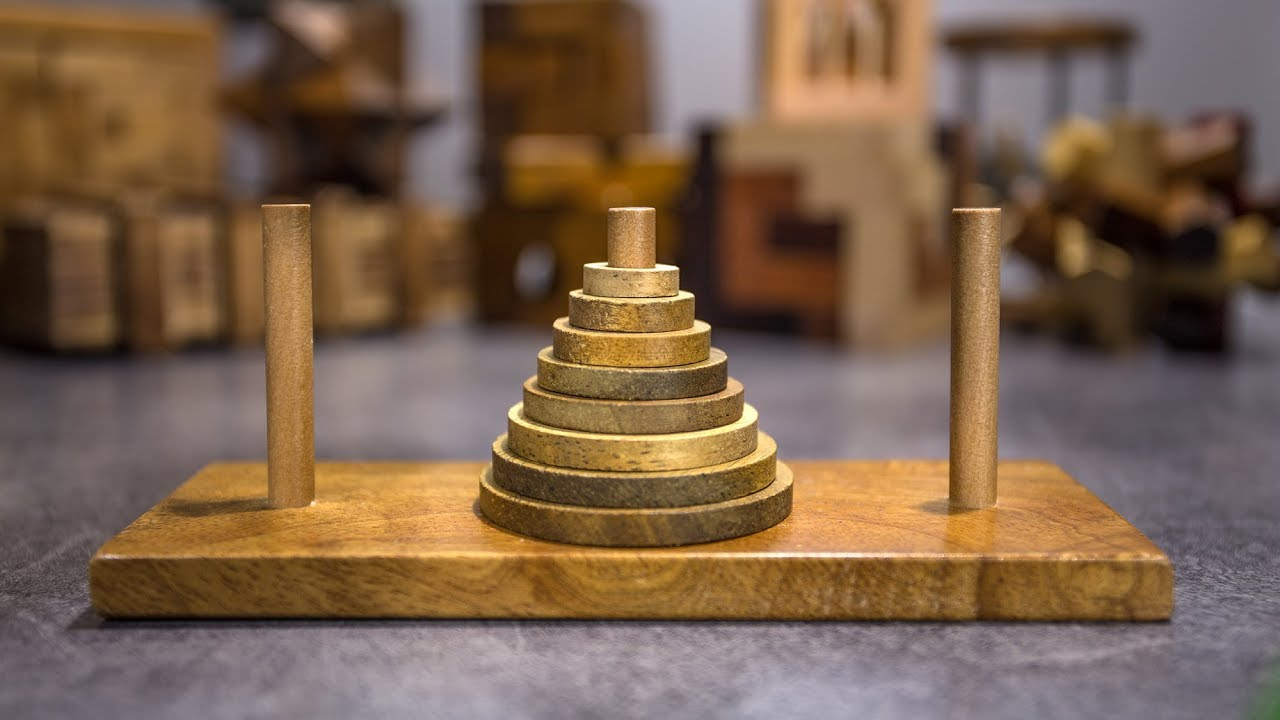
\includegraphics[width=0.5\linewidth]{tower-of-hanoi.jpg}
    \caption{Juego de las Torres de Hanoi}
    \label{fig:towers-of-hanoi}
\end{figure}

\section{Especificación del entorno de trabajo}

Definición de REAS (Rendimiento, Entorno, Actuadores, Sensores):
\begin{itemize}
    \item \textbf{Tipo de agente:} Sistema para resolución del juego Torres de Hanoi.
    \item \textbf{Medidas de rendimiento:} Cantidad de movimientos de los discos.
    \item \textbf{Entorno:} Sistema de discos y postes, es decir, el juego Torres de Hanoi.
    \item \textbf{Actuadores:} Capacidad de mover discos de un poste a otro dadas las restricciones del juego.
    \item \textbf{Sensores:} Conocimiento del estado actual del sistema de discos y postes.
\end{itemize}

\section{Propiedades del entorno de trabajo}

Definición de las propiedades del entorno de trabajo:
\begin{itemize}
    \item \textbf{Totalmente observable:} porque los sensores del agente le proporcionan acceso al estado completo del medio en cada momento.
    \item \textbf{Determinista:} porque el siguiente estado del medio esta totalmente determinado por el estado actual y la acción ejecutada por el agente.
    \item \textbf{Secuencial:} el siguiente episodio depende de las acciones que se realizaron en episodios previos.
    \item \textbf{Estático:} el entorno no puede cambiar cuando el agente esta deliberando.
    \item \textbf{Discreto:} el juego tiene estados discretos, es decir, un numero finito de estados distintos.
    \item \textbf{Agente individual:} el agente no compite ni coopera con ningún otro agente inteligente.
\end{itemize}

\section{Formulación del problema}

El problema se define formalmente por los siguientes componentes:
\begin{itemize}
    \item \textbf{Estados:} la descripción de un estado especifica la localización de cada uno de los discos en cada uno de los postes.
    \item \textbf{Estado inicial:} estado en el que todos los discos están apilados de mayor a menor radio desde la base del poste hacia arriba.
    \item \textbf{Acción:} movimiento de un disco superior $a$ en un poste $m$ a un poste $n$ siempre que en el poste $n$ no haya un disco superior $b$ de menor radio que $a$.
    \item \textbf{Función sucesor:} para un determinado estado del juego $x$, la función sucesor devuelve un conjunto de pares ordenados $<\text{acción}, \text{sucesor}>$ con todas las posibles acciones legales y el estado sucesor de ejecutarse.
    \item \textbf{Test objetivo:} estado en el que todos los discos están apilados en un poste $m$ distinto al utilizado en el estado inicial.
    \item \textbf{Espacio de estados:} definido implícitamente por el estado inicial y la función sucesor. Forma un grafo en el cual los nodos son estados y los arcos entre los nodos son acciones.
    \item \textbf{Árbol de búsqueda:} el árbol generado a partir de la expansión de nodos a partir del estado inicial (raíz del árbol) con la función sucesor.
    \item \textbf{Nodo de búsqueda:} corresponde a la raíz del árbol de búsqueda y por lo tanto es equivalente al estado inicial.
    \item \textbf{Frontera:} colección de nodos que se han generado pero todavía no se han expandido (hojas del árbol de búsqueda).
\end{itemize}

\section{Implementación de algoritmos de búsqueda}

Algoritmos de búsqueda implementados:
\begin{itemize}
    \item Búsqueda primero en profundidad
    \item Búsqueda primero en profundidad limitada
    \item Búsqueda primero en profundidad con profundización iterativa
\end{itemize}

\begin{table}[ht]
\centering
\begin{tabular}{|l|l|l|}
\hline
\textbf{Algoritmo de busqueda} & \textbf{Busqueda primero en profundidad (DFS)} & \textbf{\begin{tabular}[c]{@{}l@{}}Busqueda primero en profundidad con\\ profundizacion iterativa (IDDFS)\end{tabular}} \\ \hline
\textbf{Complejidad temporal} & $O(n^m)$ & $O(n^m)$ \\ \hline
\textbf{Complejidad espacial} & $O(bm)$ & $O(bm)$ \\ \hline
\textbf{Media del pico de memoria utilizada} & 0.2393 MB & 0.4150 MB \\ \hline
\textbf{Desviacion estandar del  pico de memoria utilizada} & 0.0019 MB & 0.0506 MB \\ \hline
\textbf{Media del tiempo de ejecucion} & 4.12 ms & 171 ms \\ \hline
\textbf{Desviacion estandar del tiempo de ejecucion} & 93.5 us & 2.9 ms \\ \hline
\textbf{Longitud de camino (diferencia con solucion optima)} & 121 (+90) & 65 (+34) \\ \hline
\end{tabular}
\end{table}

\end{document}
